\documentclass[tikz]{standalone}
\usepackage{graphicx}
\usepackage{tkz-berge}
\makeatletter
\newcommand*{\grWheelComplete}[2][]{%
  \begingroup%
  \setkeys[GR]{cl}{#1}%
  \grStar[#1]{#2}%
  \pgfmathsetcounter{tkz@gr@a}{#2-1}%
  \edef\tkz@auxctp{\thetkz@gr@a}%
  \foreach \ia in {0,...,\tkz@auxctp}%
  {\foreach \ib in {\ia,...,\tkz@auxctp}%
    {\Edge(\cmdGR@cl@prefix\ia)(\cmdGR@cl@prefix\ib)}%
  }%
  \endgroup%
}
\makeatother
\begin{document}
\begin{tikzpicture}[scale=.8]
  \GraphInit[vstyle=Shade]%
  \SetGraphShadeColor{blue!60!black!30}{blue}{white}%
  \tikzset{%
    VertexStyle/.style = {%
      shape        = circle,%
      fill          = white,%
      minimum size = 3.5cm,%
      draw%
    }%
  }%
  \SetVertexNoLabel%
  \grWheelComplete[RA=9]{6}%
  \AssignVertexLabel{a}{%
    
\includegraphics[height=25mm]{nwejm-fields-institute-logo},%
    
\includegraphics[height=25mm]{nwejm-federation-recherche-math-npdc-logo},%
    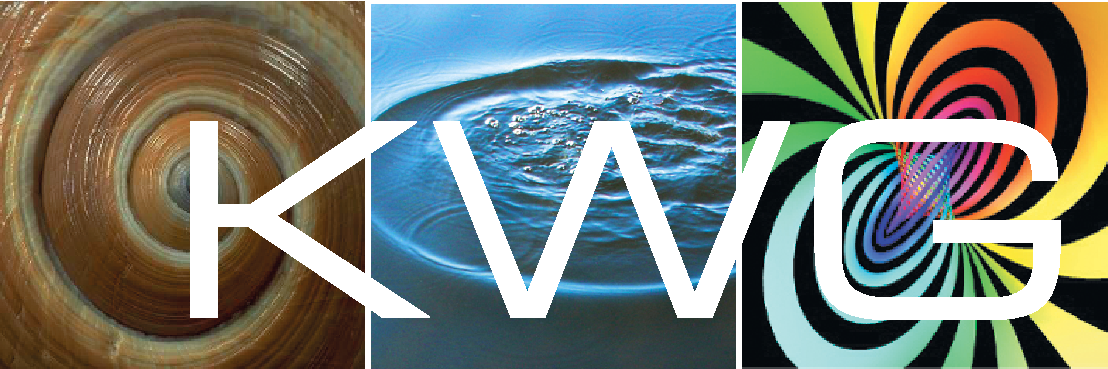
\includegraphics[height=10mm]{nwejm-kwg-logo},%
    
\includegraphics[height=20mm]{nwejm-smf-logo},%
    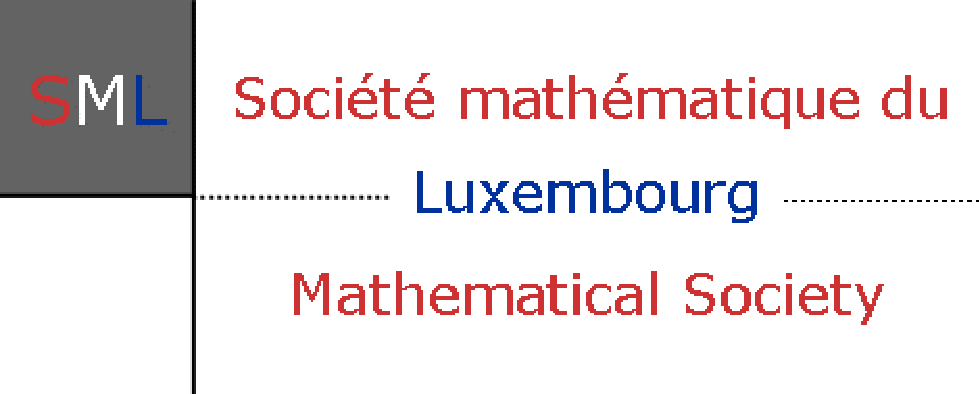
\includegraphics[height=12mm]{nwejm-sml-logo},%
    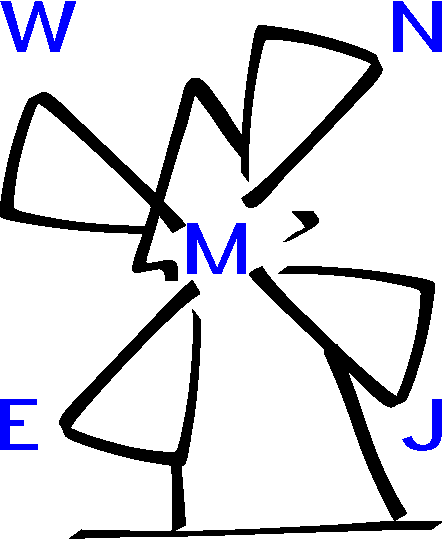
\includegraphics[height=25mm]{nwejm-logo}%
  };%
\end{tikzpicture}
\end{document}
